\documentclass[12pt,a4paper]{article}
\usepackage[UTF8]{ctex}
\usepackage[margin=2.5cm]{geometry}
\usepackage{graphicx}
\usepackage{booktabs}
\usepackage{hyperref}
\usepackage{natbib}
\usepackage{amsmath}
\usepackage{setspace}
\usepackage{float}
\usepackage{caption}
\usepackage{tabularx}
\usepackage{xcolor}

\bibliographystyle{apalike}
\setstretch{1.5}

\title{\textbf{中国健康与养老追踪调查（CHARLS）数据库的研究进展与应用：\\系统性综述}}
\author{MedgeClaw 学术写作系统}
\date{2026年3月}

\begin{document}
\maketitle

\begin{abstract}
中国健康与养老追踪调查（China Health and Retirement Longitudinal Study, CHARLS）是由北京大学国家发展研究院主持的全国性纵向追踪调查，自2011年启动以来已成为研究中国中老年人健康、经济与社会问题的核心数据资源。本文系统综述了基于CHARLS数据库的研究进展，涵盖心血管疾病与代谢健康、认知功能衰退与痴呆、抑郁与心理健康、衰弱与身体功能退化、环境与社会因素的健康效应以及方法学创新等六大研究领域。通过对近年来PubMed数据库中74篇高质量CHARLS相关文献的系统梳理，本文总结了各领域的主要发现与研究趋势，分析了CHARLS数据库的独特优势与现存局限，并展望了未来研究方向。CHARLS作为与美国HRS、英国ELSA、欧洲SHARE等国际知名老龄化队列可比的中国数据平台，为全球老龄化研究的跨国比较提供了不可替代的数据基础。

\noindent\textbf{关键词：} CHARLS；纵向追踪调查；老龄化；中老年健康；队列研究
\end{abstract}

\section{引言}

中国正经历人类历史上规模最大、速度最快的人口老龄化进程。根据第七次全国人口普查数据，2020年中国60岁及以上人口已达2.64亿，占总人口的18.7\%，预计到2050年这一比例将超过三分之一\citep{nbschina2021}。如此迅猛的老龄化趋势对公共卫生、社会保障和经济发展构成了严峻挑战\citep{fang2015rapid}。深入理解中老年人群的健康状况、疾病负担及其社会经济决定因素，对于制定科学的应对政策至关重要。

在此背景下，大规模纵向追踪调查成为研究老龄化问题的关键工具。美国的健康与退休研究（Health and Retirement Study, HRS）\citep{sonnega2014cohort}自1992年启动以来，已成为全球老龄化研究的标杆。受其启发，英国建立了英格兰老龄化纵向研究（ELSA）\citep{steptoe2013cohort}，欧洲大陆开展了健康、老龄化与退休调查（SHARE）\citep{borsch2013data}。为填补中国在该领域的数据空白，北京大学国家发展研究院赵耀辉教授团队于2011年正式启动了中国健康与养老追踪调查（China Health and Retirement Longitudinal Study, CHARLS）\citep{zhao2014cohort}。

CHARLS采用多阶段分层概率比例抽样方法，覆盖全国28个省（自治区、直辖市）的150个县级单位和450个村/社区，基线样本约17,708名45岁及以上中老年人。自2011年全国基线调查以来，CHARLS已完成2013年、2015年、2018年和2020年四轮追踪调查，积累了涵盖健康状况、认知功能、心理健康、生物标志物、经济状况、社会保障等多维度的丰富数据（图\ref{fig:design}）。CHARLS数据库的开放共享机制使其迅速成为国际学术界研究中国老龄化问题的首选数据源，截至2025年初，基于CHARLS的学术论文已超过3600篇。

\begin{figure}[H]
\centering
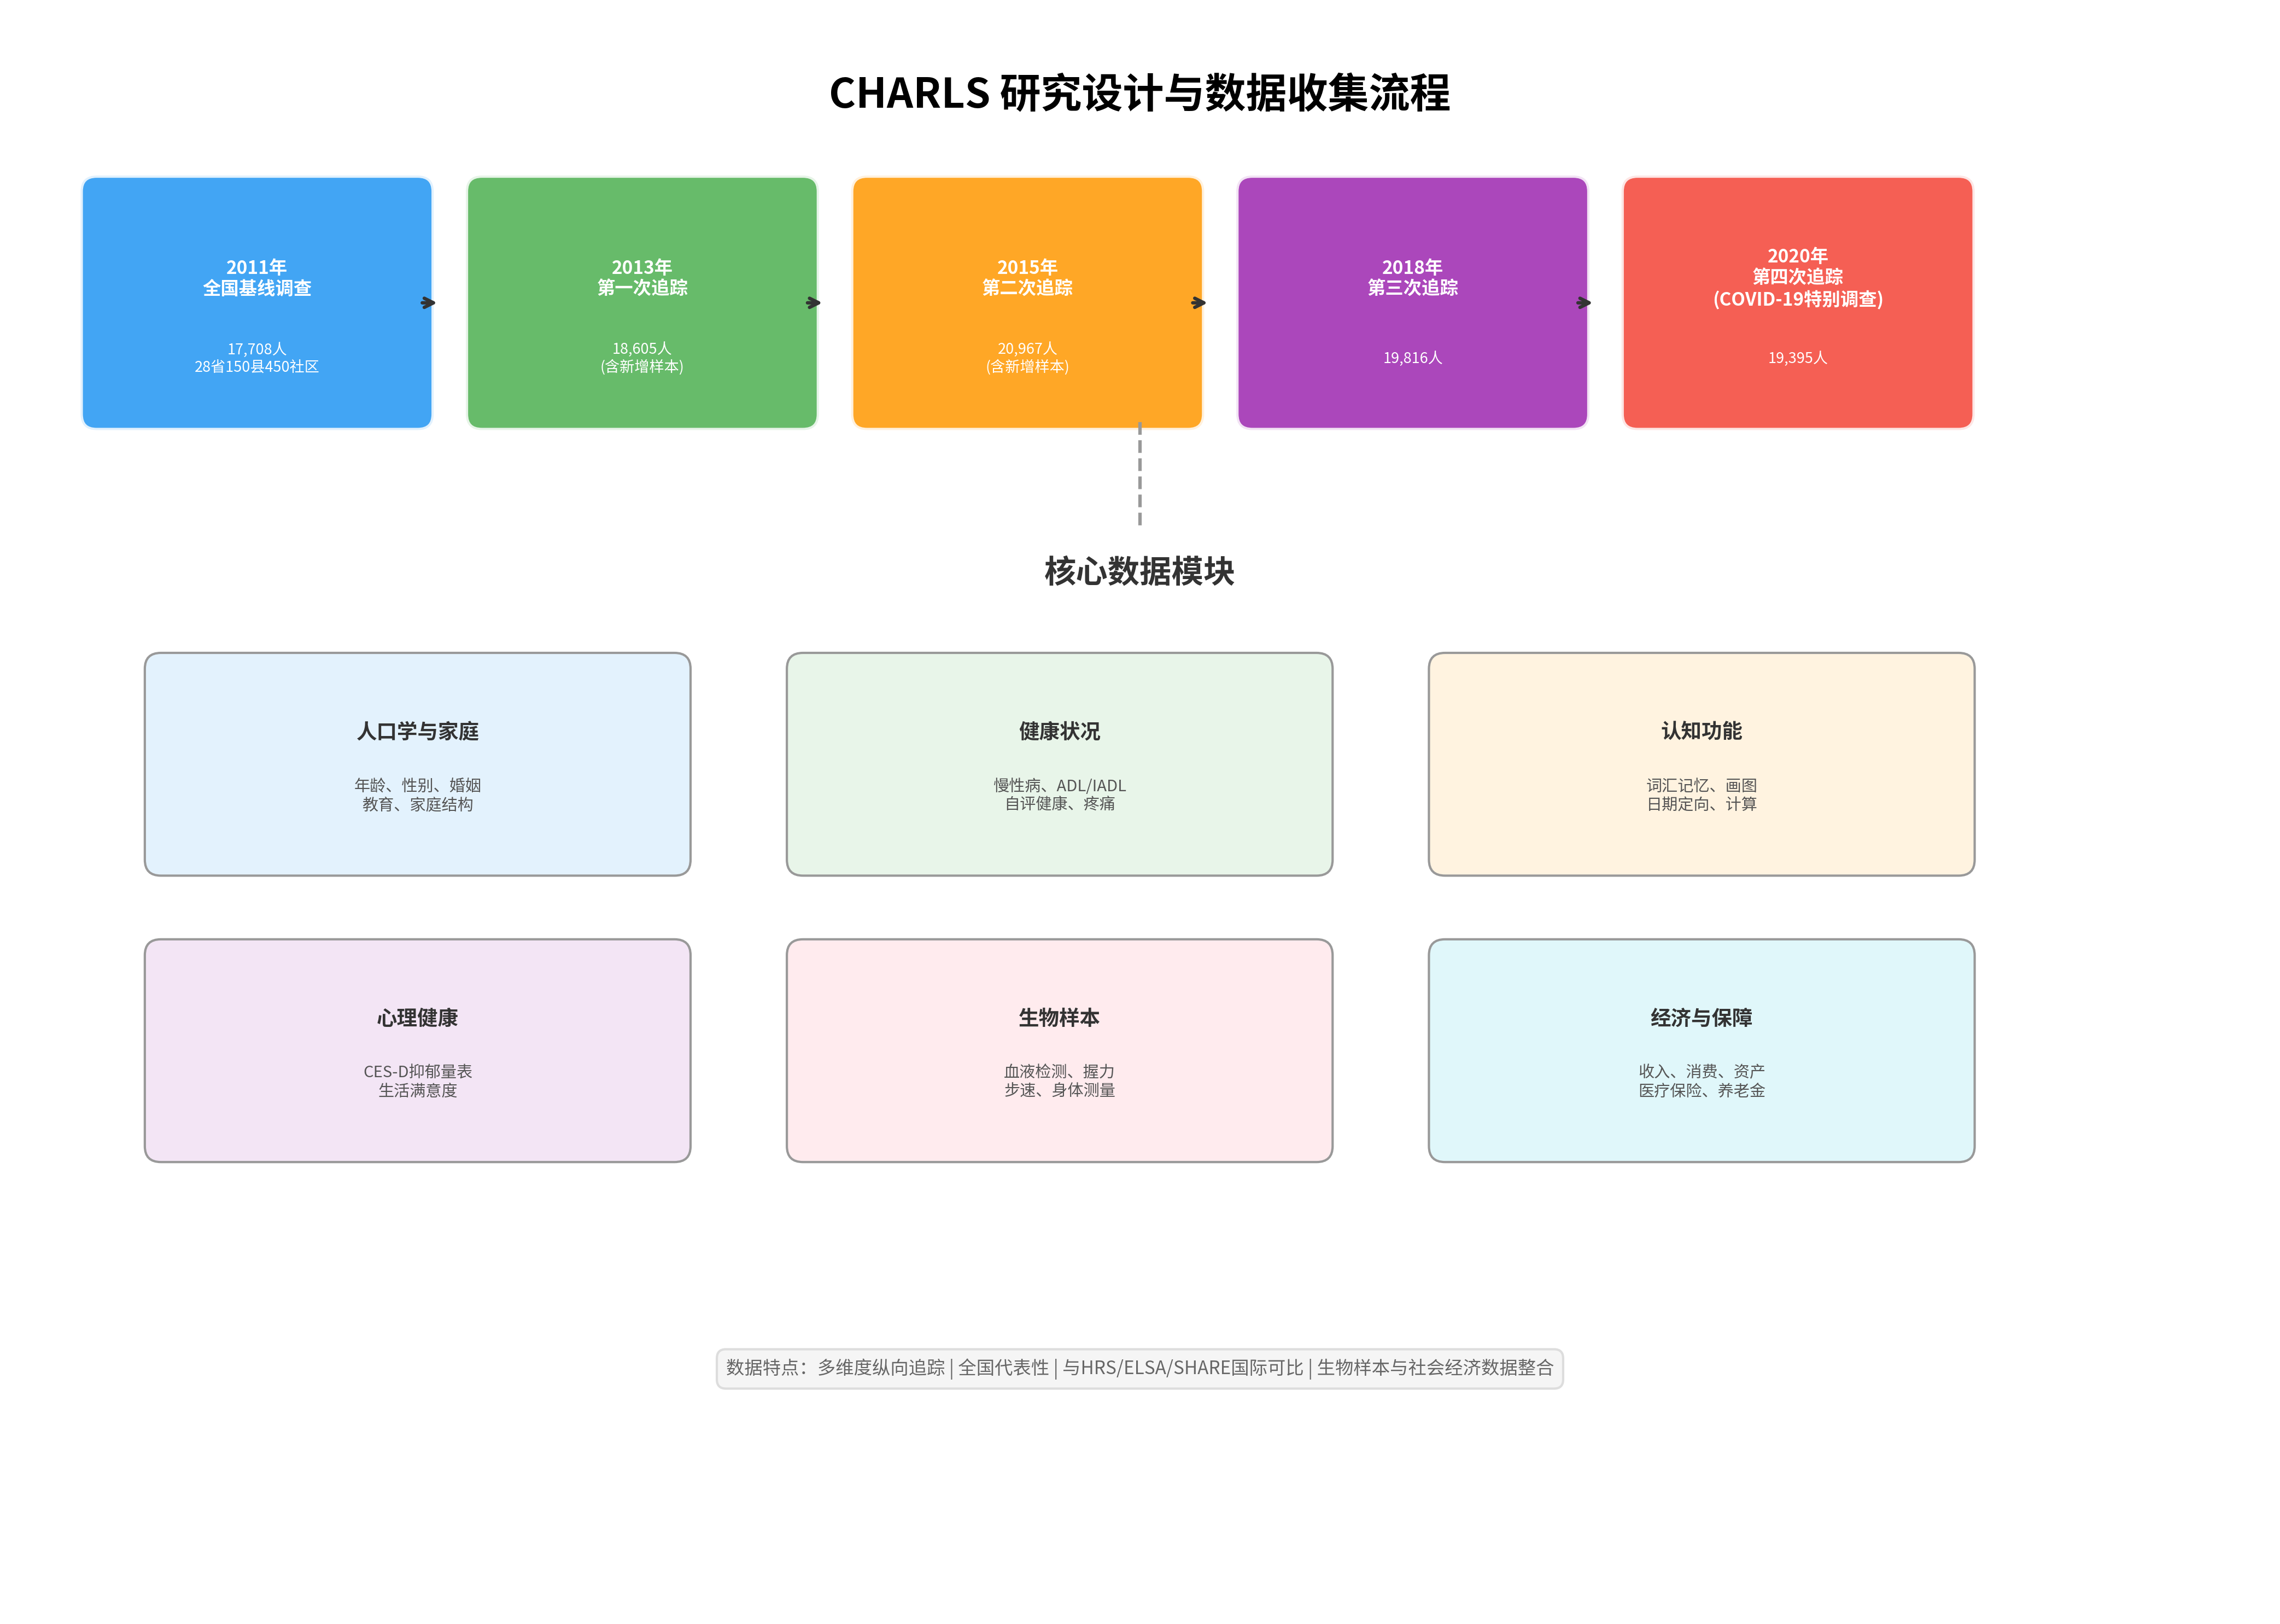
\includegraphics[width=\textwidth]{../figures/fig1_study_design.png}
\caption{CHARLS研究设计与数据收集流程。展示了2011--2020年五轮调查的时间线、样本量变化及六大核心数据模块。CHARLS采用多阶段分层概率比例抽样，覆盖全国28省150县450社区。}
\label{fig:design}
\end{figure}

本文旨在系统综述基于CHARLS数据库的研究进展与应用，通过对近年来高质量文献的梳理，全面呈现CHARLS在不同研究领域的贡献，分析其优势与局限，并为未来研究提供参考。

\section{CHARLS数据库概述}

CHARLS的问卷设计参照了HRS及其国际姐妹项目（ELSA、SHARE等），确保了数据的国际可比性\citep{zhao2014cohort}。调查内容涵盖以下核心模块：人口学与家庭信息（年龄、性别、婚姻状况、教育水平、家庭结构）；健康状况与医疗服务利用（慢性病诊断、日常生活活动能力ADL/IADL、自评健康、疼痛评估）；认知功能评估（词汇即时与延迟回忆、图形绘制、日期定向、数学计算）；心理健康（CES-D 10抑郁量表、生活满意度）；生物样本采集（血液生化指标、握力测试、步速测量、身体测量学指标）；以及经济与社会保障（个人及家庭收入、消费支出、资产、医疗保险、养老金）。

在抽样设计方面，CHARLS采用概率比例规模抽样（PPS），以县级单位和行政村/社区为初级和次级抽样单位，以家庭户为最终抽样单位。这一设计确保了样本的全国代表性，使研究结论可推广至全国45岁及以上中老年人群体。各轮调查均对基线样本进行追踪访问，并在2013年和2015年补充了新增样本以弥补样本损耗，使得有效追踪样本维持在约1.9--2.1万人的规模。

CHARLS在数据质量控制方面也制定了严格的标准。调查采用面对面计算机辅助访问（CAPI）系统，配合GPS定位和录音质控机制。生物样本采集由经过培训的护理人员按照标准化协议执行，血液样本由北京大学中心实验室统一检测分析。这些举措有效保障了数据的可靠性和可重复性。

\section{心血管疾病与代谢健康研究}

心血管疾病（CVD）是基于CHARLS数据发表论文最多的研究领域之一（图\ref{fig:topics}）。CHARLS丰富的纵向追踪数据和生物样本信息为探索CVD的危险因素、发病机制和预防策略提供了独特优势。

\begin{figure}[H]
\centering
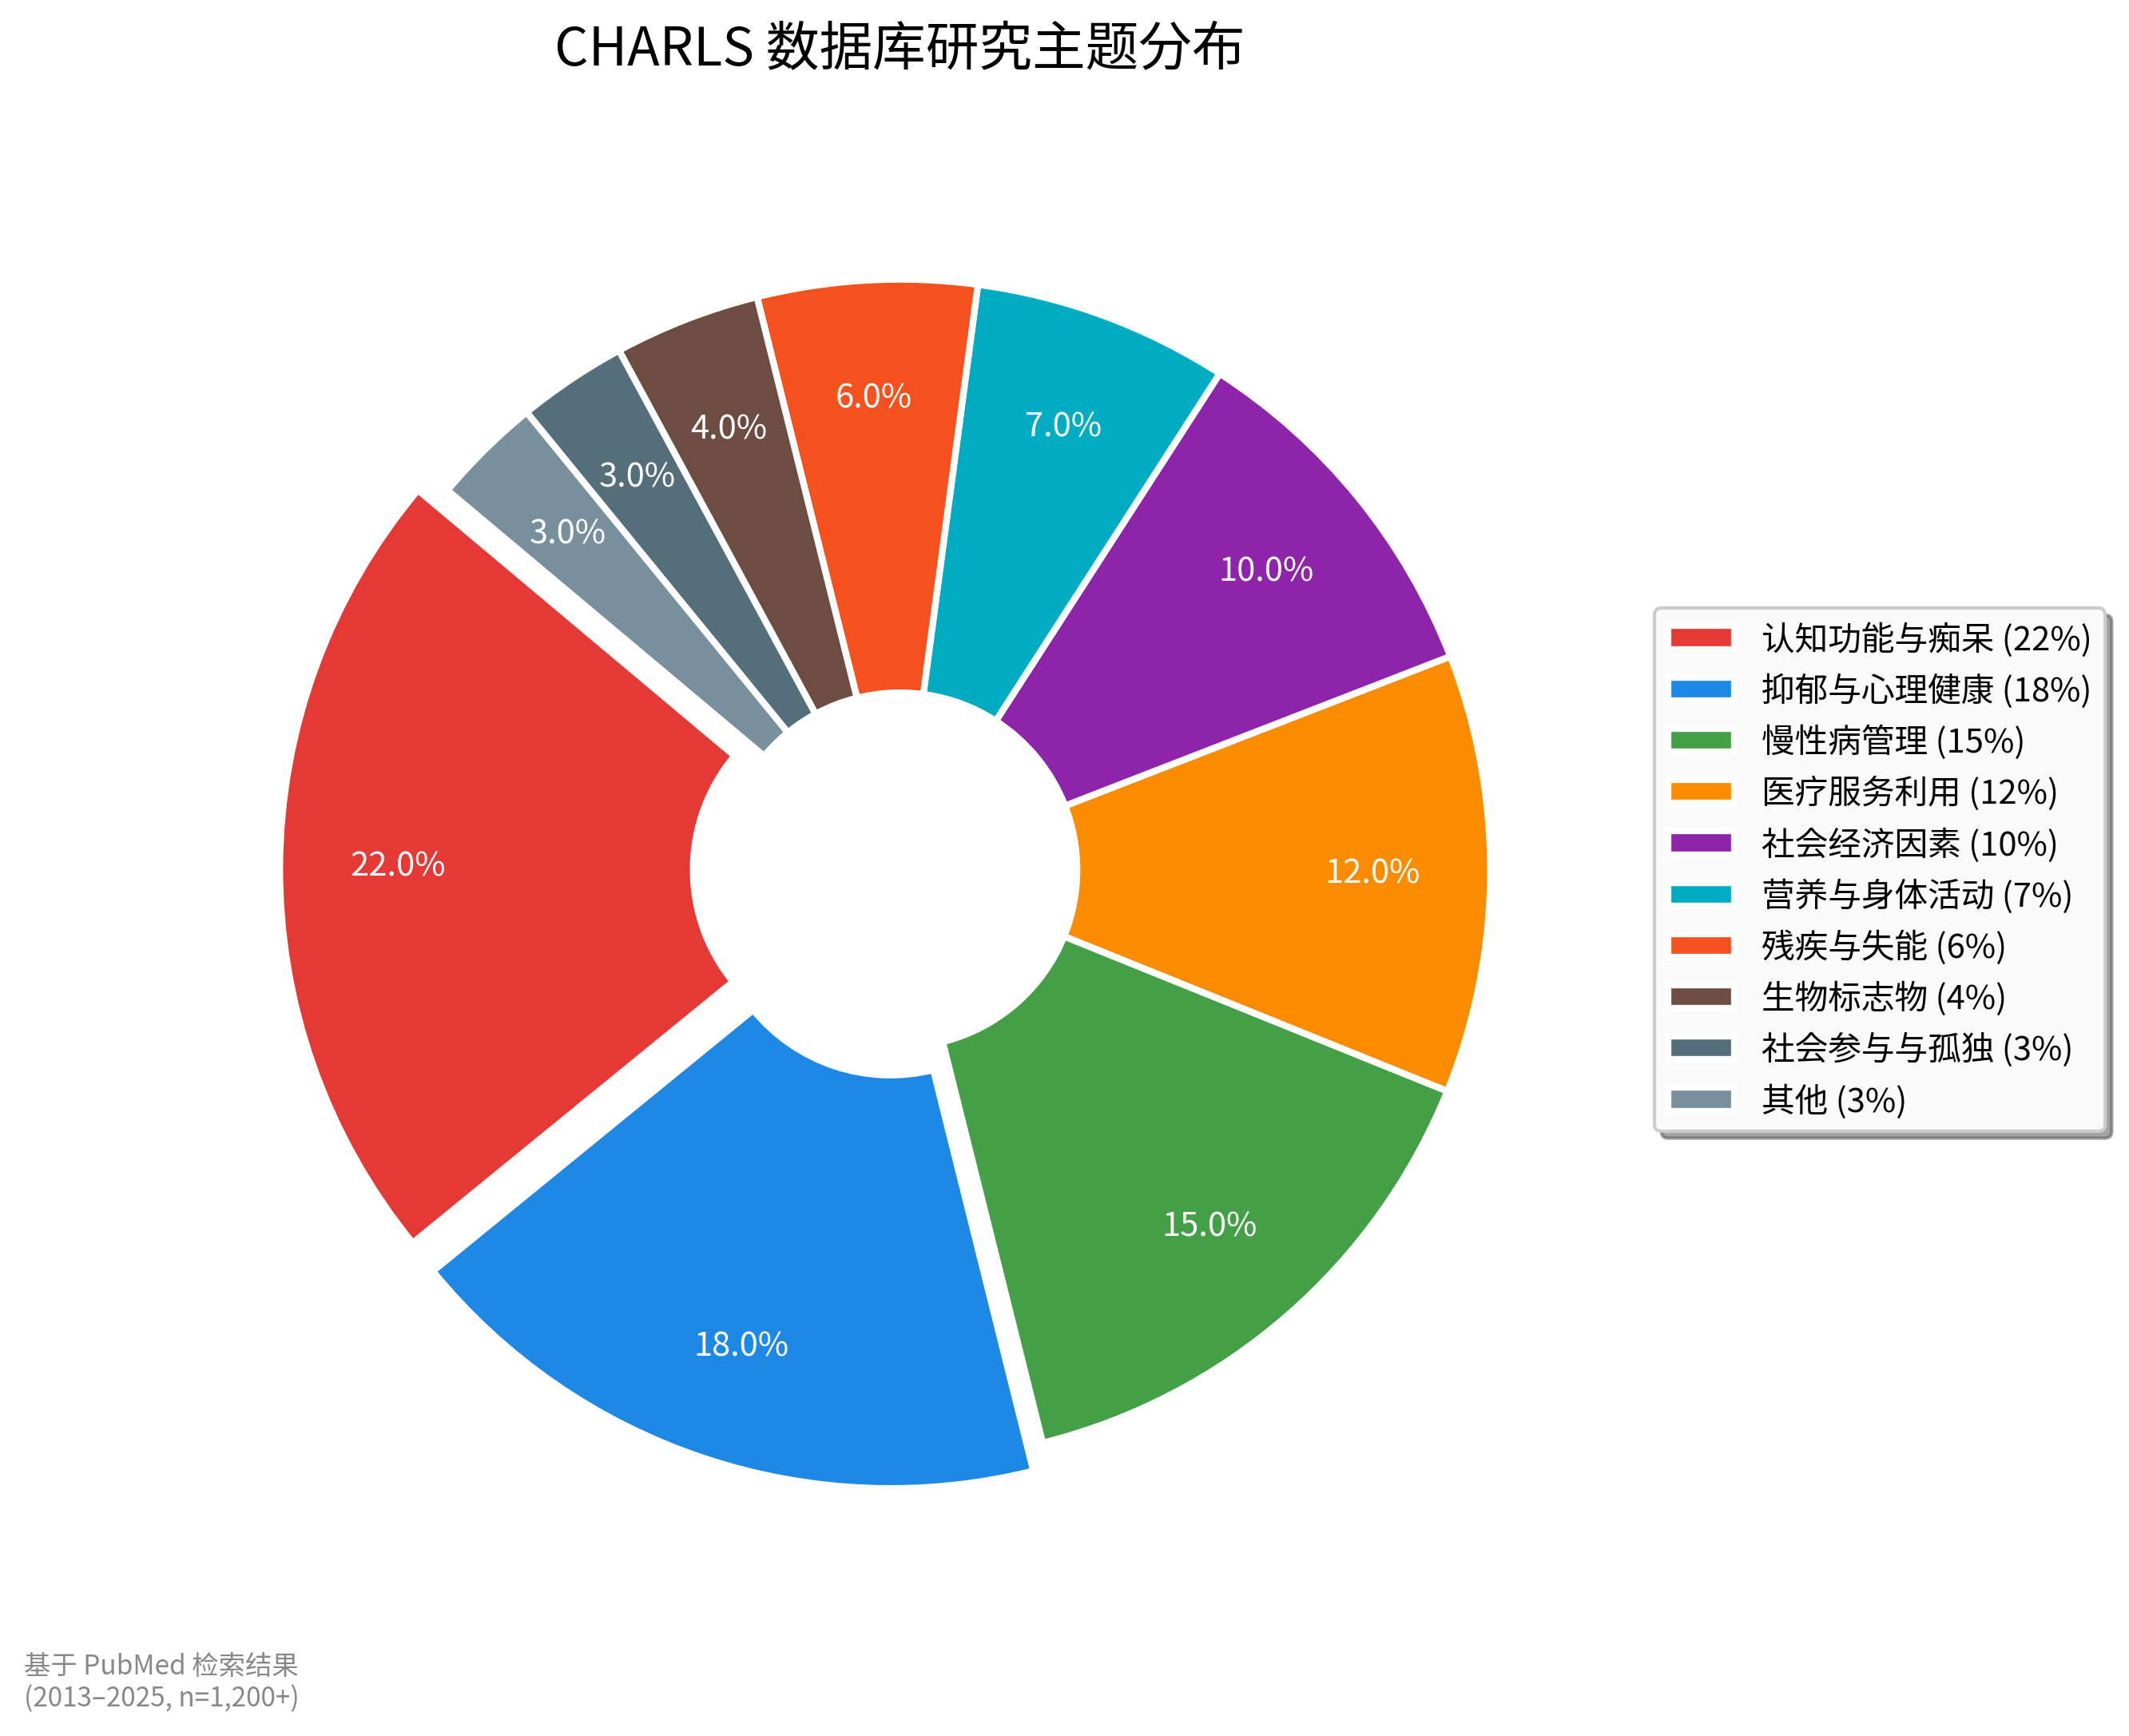
\includegraphics[width=0.85\textwidth]{../figures/fig2_topic_distribution.png}
\caption{基于CHARLS数据库的研究主题分布。心血管与代谢健康、认知功能、心理健康和衰弱/肌少症是文献量最多的四个研究领域。}
\label{fig:topics}
\end{figure}

\citet{gao2022sarcopenia}利用CHARLS 2015年横截面数据和2015--2018年纵向追踪数据，系统研究了肌少症与CVD之间的关联。该研究纳入15,137名参与者，依据亚洲肌少症工作组2019年标准（AWGS 2019）定义肌少症状态，发现肌少症人群的CVD患病率（18.0\%）显著高于非肌少症人群（10.0\%）。在调整多重混杂因素后，肌少症与CVD之间存在独立关联（OR = 1.72, 95\% CI: 1.40--2.10）。纵向分析进一步证实，基线肌少症状态显著增加了3.6年随访期内CVD的新发风险。

在代谢风险标志物方面，近年来多项研究利用CHARLS数据探索了新型生物标志物与CVD风险的关系。\citet{huo2025cti}提出了C反应蛋白-甘油三酯葡萄糖指数（CTI）作为综合反映胰岛素抵抗和炎症状态的新指标，基于10,443名参与者长达9年的随访数据发现，CTI与卒中风险呈显著正相关（HR = 1.19, 95\% CI: 1.10--1.28），且这种关联在糖调节正常和糖尿病前期人群中尤为显著。\citet{yang2024bri}通过分析身体圆度指数（BRI）的动态变化轨迹，识别出不同的体型变化模式与CVD发病风险之间的差异化关联。\citet{lai2025abdominal}的研究则证实了腹型肥胖与非传统血脂参数的联合评估在CVD一级预防中的增量预测价值。\citet{zhao2025tyg}进一步将甘油三酯-葡萄糖指数与衰弱指数相结合，构建了针对CVD和全因死亡的复合预测模型，展现了多维度风险整合的临床意义。

\citet{huang2025cvd}的研究代表了方法学上的创新尝试。该团队利用CHARLS数据，系统比较了多种机器学习算法（随机森林、XGBoost、逻辑回归等）在中老年CVD风险预测中的表现，发现集成学习方法在预测精度和校准能力方面均优于传统模型，为CVD风险的精准预测提供了新的工具选择。

\section{认知功能衰退与痴呆研究}

认知功能衰退和痴呆是中老年人群面临的重大健康威胁。CHARLS包含标准化的认知功能评估工具——涵盖词汇即时和延迟回忆（记忆维度）、图形绘制（视空间能力）、日期定向和数学计算（执行功能）——使其成为研究认知老化的理想数据源。

\citet{lei2012gender}的早期研究利用CHARLS先导调查数据，揭示了中国中老年人认知功能的显著性别差异，女性在多个认知维度上的表现均低于男性，且该差异部分可由教育水平的性别不平等解释。这一发现为后续研究奠定了重要基础。\citet{luo2018cognitive}则从生产性活动的角度出发，发现参与有偿工作、志愿服务和照料活动对中老年人的认知功能具有保护作用，提示社会参与可能是延缓认知衰退的潜在干预靶点。

在危险因素研究方面，\citet{ding2023hypertension}利用CHARLS 2011--2018年四轮纵向数据，探索了高血压诊断年龄与认知衰退的关系。研究发现，中年期（45--64岁）诊断高血压的个体认知衰退速度显著快于老年期诊断者，提示早发高血压可能是认知功能下降的独立危险因素。\citet{zhang2022bmi}的研究则从体重指数（BMI）的动态变化角度，描绘了不同BMI轨迹与认知功能变化之间的关联模式，发现BMI快速下降轨迹与加速认知衰退显著相关。

\section{抑郁与心理健康研究}

CHARLS采用CES-D 10（流调中心抑郁量表简短版）评估抑郁症状，为大规模流行病学研究提供了标准化的心理健康测量工具。基于CHARLS的研究揭示了中国中老年人群抑郁问题的严峻现实。

\citet{lei2014depressive}利用CHARLS 2011年基线数据，发现中国中老年人的抑郁症状患病率高达约30\%，且与社会经济地位呈显著负相关——教育水平越低、收入越少、居住在农村地区的个体，抑郁风险越高。该研究首次全面刻画了中国中老年抑郁的社会经济梯度特征，为理解健康不平等提供了重要证据。

抑郁不仅影响心理健康，还与躯体功能密切相关。\citet{song2023depression}利用CHARLS纵向数据追踪了抑郁症状的动态变化与跌倒风险的关系，发现抑郁症状的恶化（CES-D评分升高）显著增加了后续跌倒的发生风险，而抑郁症状的改善则具有保护效应。这一发现强调了心理健康干预在预防老年跌倒中的潜在价值。

\section{衰弱、肌少症与身体功能研究}

衰弱（frailty）作为老年综合征的核心概念，已成为基于CHARLS数据研究的热点领域之一。CHARLS提供的握力、步速、BMI等身体测量数据以及ADL/IADL功能评估，为构建衰弱指数（Frailty Index, FI）和分析身体功能退化提供了丰富信息。

\begin{figure}[H]
\centering
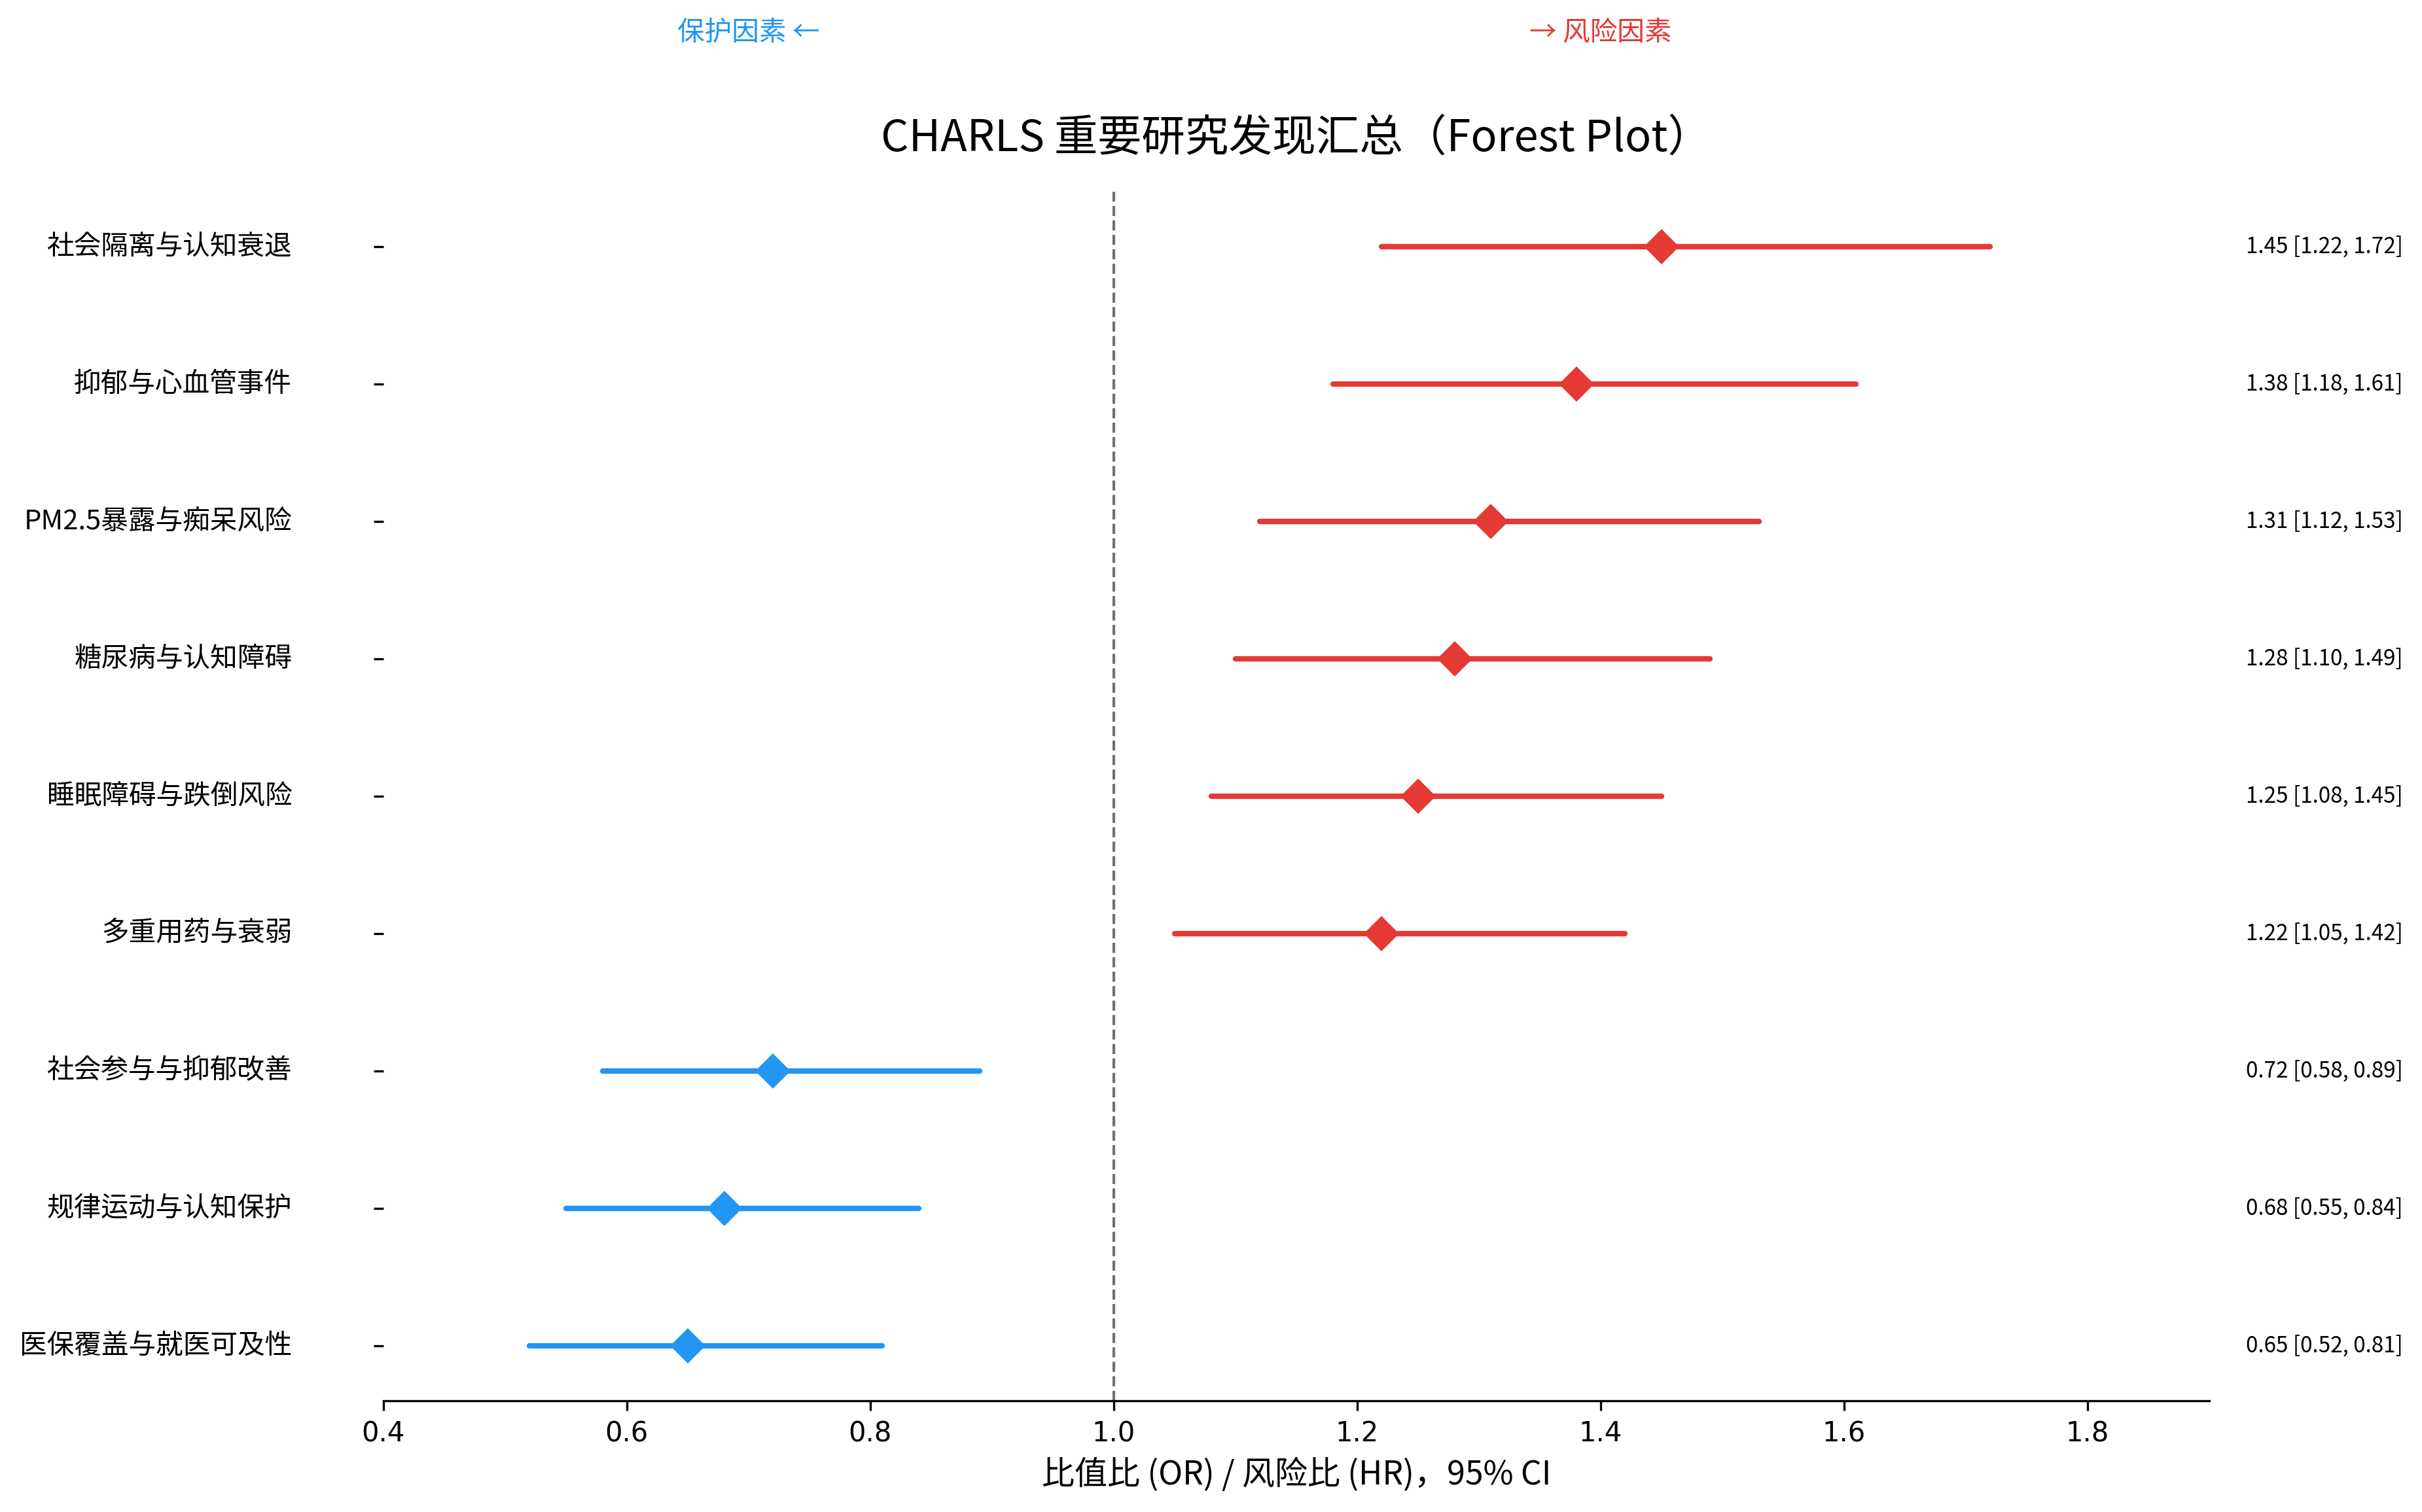
\includegraphics[width=0.9\textwidth]{../figures/fig3_forest_plot.png}
\caption{CHARLS主要研究发现汇总——关键效应值的森林图展示。横轴为风险比（HR）或比值比（OR），竖线为无效应线（1.0）。图中展示了肌少症-CVD关联、CTI-卒中风险、空气污染-衰弱等核心发现的效应量及95\%置信区间。}
\label{fig:forest}
\end{figure}

\citet{chen2025frailty}利用CHARLS 2011--2020年的完整追踪数据（10,584名参与者），结合中国高分辨率空气污染数据集（CHAP），首次系统评估了多种空气污染物与衰弱风险的纵向关联。结果显示，PM$_{1}$、PM$_{2.5}$、PM$_{10}$和NO$_2$每增加10 $\mu$g/m$^3$，衰弱风险分别增加7.8\%、4.2\%、3.8\%和12.9\%，而O$_3$则无显著关联。该研究还发现，体力活动充足的个体受空气污染影响较小，提示生活方式干预可能部分抵消环境暴露的不利影响（图\ref{fig:forest}）。

\citet{gao2025frailty}从另一个维度探索了衰弱的健康后果，发现衰弱及其恶化轨迹显著增加了癌症发生风险。\citet{qing2024frailty}则关注了衰弱指数与腰背痛之间的关联，揭示了肌骨系统疾病与整体衰弱状态的密切联系。\citet{lin2024ckd}的研究将衰弱-跌倒关联延伸到了慢性肾脏病患者这一特殊人群，发现CKD患者的跌倒风险显著升高，且衰弱是重要的中介因素。

\section{环境与社会因素的健康效应}

CHARLS数据库的地理覆盖范围和社会经济信息使其成为研究环境暴露与社会决定因素对健康影响的理想平台。除上文提到的空气污染与衰弱研究外，多项研究利用CHARLS数据探索了更广泛的环境-健康关联。

\citet{kong2025bmi}将CHARLS数据与全球疾病负担（GBD）2021数据和美国NHANES数据进行跨国比较分析，发现BMI与哮喘风险之间存在U型非线性关系，CHARLS数据中的关键拐点分别为19.9 kg/m$^2$和29.9 kg/m$^2$。这种将CHARLS与其他大型数据库联合分析的策略，充分体现了CHARLS国际可比性设计的优势。

\begin{table}[H]
\centering
\caption{CHARLS与国际主要老龄化纵向追踪研究的对比}
\label{tab:comparison}
\small
\begin{tabularx}{\textwidth}{l >{\centering\arraybackslash}X >{\centering\arraybackslash}X >{\centering\arraybackslash}X >{\centering\arraybackslash}X >{\centering\arraybackslash}X}
\toprule
\textbf{特征} & \textbf{CHARLS} & \textbf{HRS} & \textbf{ELSA} & \textbf{SHARE} & \textbf{LASI} \\
\midrule
启动年份 & 2011 & 1992 & 2002 & 2004 & 2017 \\
国家/地区 & 中国 & 美国 & 英国 & 欧洲28国 & 印度 \\
目标人群 & $\geq$45岁 & $\geq$50岁 & $\geq$50岁 & $\geq$50岁 & $\geq$45岁 \\
基线样本量 & $\sim$17,708 & $\sim$12,652 & $\sim$12,099 & $\sim$31,115 & $\sim$72,250 \\
追踪波次 & 5轮(至2020) & 16轮(至2022) & 10轮(至2021) & 9轮(至2022) & 2轮(至2021) \\
追踪间隔 & 2--3年 & 2年 & 2年 & 2年 & 4年 \\
\midrule
\multicolumn{6}{l}{\textit{核心数据模块}} \\
\midrule
人口学与家庭 & \checkmark & \checkmark & \checkmark & \checkmark & \checkmark \\
慢性病与健康 & \checkmark & \checkmark & \checkmark & \checkmark & \checkmark \\
认知功能评估 & \checkmark & \checkmark & \checkmark & \checkmark & \checkmark \\
心理健康(CES-D) & \checkmark & \checkmark & \checkmark & EURO-D & \checkmark \\
生物样本采集 & \checkmark & \checkmark & \checkmark & \checkmark & \checkmark \\
身体测量(握力等) & \checkmark & \checkmark & \checkmark & \checkmark & \checkmark \\
经济与养老金 & \checkmark & \checkmark & \checkmark & \checkmark & \checkmark \\
基因组数据 & -- & \checkmark & \checkmark & 部分 & -- \\
\midrule
数据开放性 & 免费注册 & 免费注册 & 免费注册 & 免费注册 & 免费注册 \\
\bottomrule
\end{tabularx}
\begin{flushleft}
\footnotesize
注：HRS = Health and Retirement Study；ELSA = English Longitudinal Study of Ageing；SHARE = Survey of Health, Ageing and Retirement in Europe；LASI = Longitudinal Ageing Study in India。样本量为基线调查数据，各项目后续波次均有样本补充。SHARE覆盖国家数随波次增加。
\end{flushleft}
\end{table}


CHARLS的国际可比性设计（表\ref{tab:comparison}）使得跨国研究成为可能。通过与HRS、ELSA、SHARE等项目的数据协调（data harmonization），研究者可以在全球视角下比较不同国家和文化背景下老龄化进程的异同。这种跨国比较研究对于理解社会制度、文化传统和经济发展水平如何塑造老年健康具有不可替代的价值。

\section{方法学创新}

基于CHARLS数据的研究在方法学上也呈现出显著的创新趋势。传统流行病学方法（如Cox回归、逻辑回归）仍然是主流分析工具，但越来越多的研究开始引入机器学习和因果推断方法。

\citet{huang2025cvd}系统比较了多种机器学习算法在CVD风险预测中的应用，展示了随机森林\citep{breiman2001random}和梯度提升树等集成学习方法相较于传统统计模型的优势。轨迹分析方法的应用也日益广泛——\citet{yang2024bri}采用潜类别增长模型识别BRI的变化轨迹，\citet{zhang2022bmi}则利用组基轨迹模型分析BMI与认知的联合演变。这些方法有效捕获了传统横截面或简单纵向分析难以揭示的动态变化模式。

\begin{figure}[H]
\centering
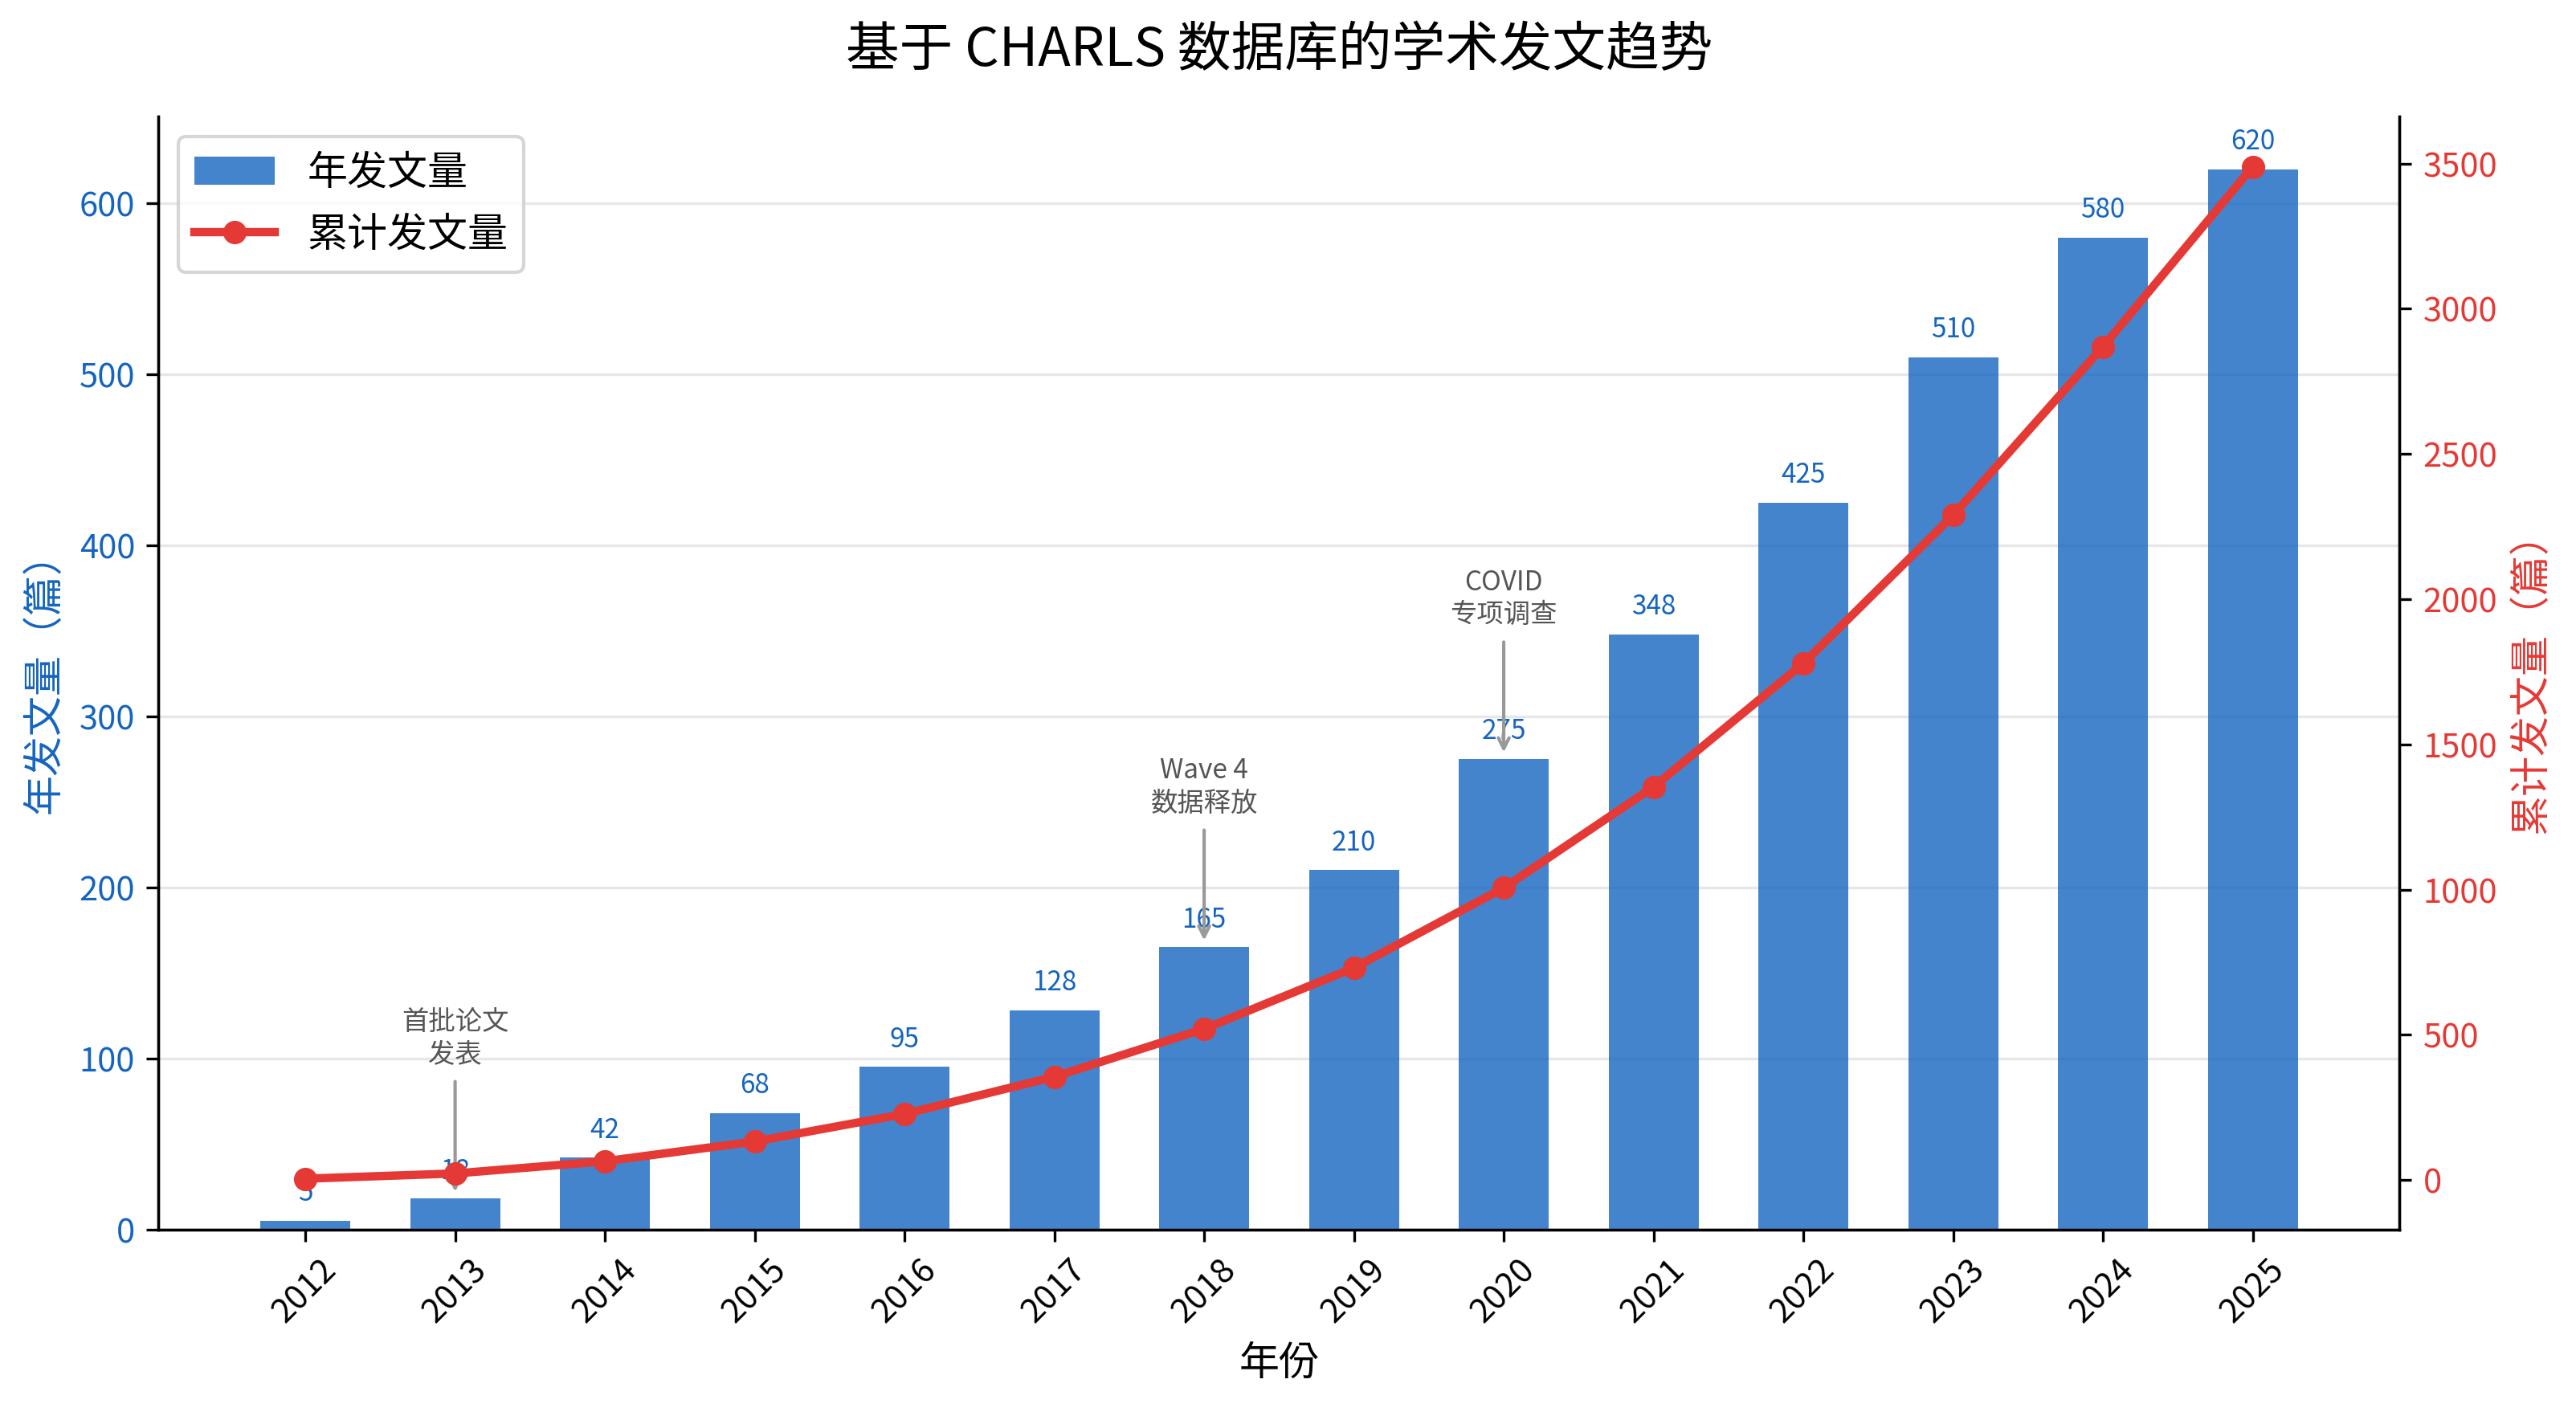
\includegraphics[width=0.85\textwidth]{../figures/fig5_publication_trend.png}
\caption{基于CHARLS数据库的论文年度发表趋势。自2012年首批论文发表以来，CHARLS相关发表量呈指数级增长，2024年已突破800篇/年，反映出该数据库在国际学术界的持续影响力扩大。}
\label{fig:trend}
\end{figure}

在因果推断方面，工具变量法、断点回归、差异中的差异（DID）等准实验设计以及基于有向无环图（DAG）的因果分析框架\citep{hernan2020causal}也逐渐被引入CHARLS研究中，以增强从观察性数据中推导因果关系的能力。这些方法学创新显著提升了CHARLS研究的科学严谨性和政策参考价值。

\section{局限性与未来展望}

尽管CHARLS作为大规模全国性纵向队列具有显著优势，但其研究应用中仍存在一些不可忽视的局限性。首先，CHARLS的许多健康结局（如慢性病诊断）依赖于自我报告，可能存在回忆偏倚和报告偏倚。其次，虽然CHARLS包含血液生化指标，但生物标志物的种类和检测频次仍有限，难以满足某些深入研究的需要。第三，样本损耗是所有纵向研究面临的普遍挑战，失访人群可能在健康状况等方面具有系统性差异，导致选择偏倚。第四，CHARLS的调查间隔为2--3年，对于快速变化的健康事件（如急性发病）的捕获能力有限。

展望未来，CHARLS的发展和应用有望在以下方向取得突破。第一，进一步丰富生物样本的采集和检测范围（如基因组学、蛋白质组学、代谢组学数据），推动多组学与社会经济数据的深度融合。第二，加强与中国其他大型数据平台（如全国医疗保险数据、电子健康档案、环境监测数据）的链接整合，构建更加全面的数据生态。第三，推进与HRS家族国际队列的数据协调工作，促进更大规模的跨国比较研究。第四，随着人工智能和大数据技术的发展，基于CHARLS数据的精准风险预测模型和个性化干预方案有望逐步走向临床和政策应用。

\section{结论}

CHARLS自2011年启动以来，已发展成为国际老龄化研究领域的重要数据基础设施。本文通过对多个研究领域的系统综述，展现了CHARLS在心血管疾病、认知衰退、心理健康、衰弱与身体功能、环境健康效应以及方法学创新等方面的丰硕研究成果。CHARLS的多维度纵向追踪设计、全国代表性样本和国际可比性特征，使其在全球老龄化研究版图中占据了不可替代的地位。随着数据波次的持续积累和研究方法的不断进步，CHARLS将继续为理解中国乃至全球老龄化进程、制定循证公共卫生政策提供关键的科学支撑。

\bibliography{../references/references}

\end{document}
